\section{Durchführung}
\label{sec:Durchführung}
Der experimentelle Aufbau ist in Abb. \ref{fig:aufbau} zu sehen.
\begin{figure}
    \centering
    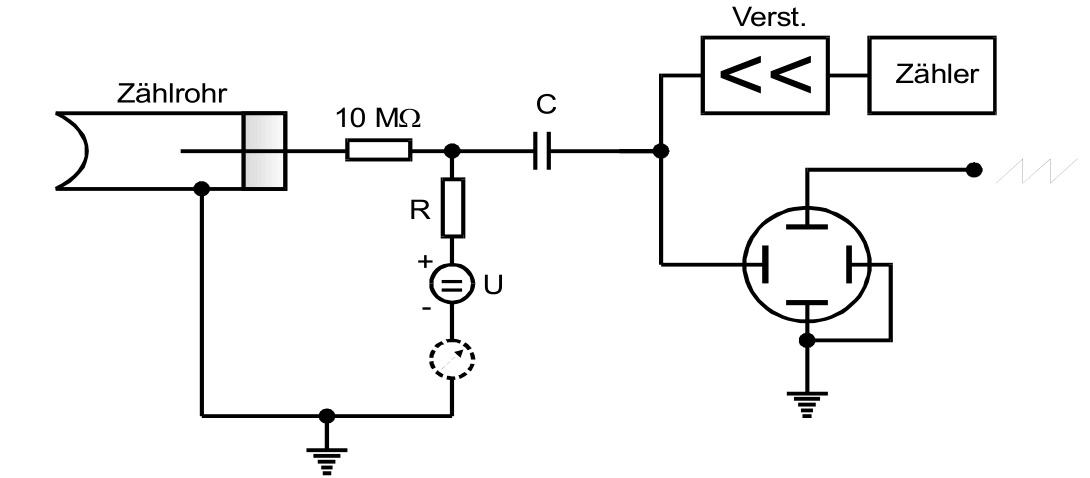
\includegraphics[width=0.8\textwidth]{content/data/aufbau.jpg}
    \caption{Schematische Darstellung der Messapparatur. \cite[7]{anleitung}}
    \label{fig:aufbau}
\end{figure}
Die gesammelte Ladung $Q$ auf dem Zähldraht fließt in den Widerstand $R$ und erzeugt dort ein Spannungsimpuls.
Der Impuls wird über den Kondensator ausgekoppelt und verstärkt.
Das Zählgerät registriert den Impuls.
Zusätzlich kann dieser auch mithilfe eines Oszillographen sichtbar gemacht werden.
\\
Zuerst soll die Geiger-Müller Charakteristik aufgenommen werden.
Dazu wird eine $\beta$-Quelle vor das Fenster des Zählrohrs gestellt.
Dann wird die Zählrate in Abhängigkeit der Spannung gemessen.
Die Spannung wird in $\Delta U = \SI{10}{\volt}$-Schritten im Bereich von $\SI{320}{\volt}$ bis $\SI{700}{\volt}$ gemessen.
Die Intensität darf nicht über $\SI{100}{\text{Imp}/\second}$ steigen, damit das Zählrohr nicht durch Dauerentladungen beschädigt wird.
Die Integrationszeit beträgt $\SI{60}{\second}$.
Es ist wichtig eine hohe Anzahl an Impulsen zu messen, damit die gesammelte Ladung nicht mehr von der Primärionisation abhängt.
Bei $\SI{350}{\volt}$ und jeder weiteren $5$-ten Messung wird der Zählstrom $I$ am Amperemeter abgelesen.
Die Ablesegenauigkeit beträgt hier $\Delta I = \SI{0.05}{\micro \ampere}$.
\\
Als nächstes wird die Totzeit bestimmt.
Hier wird die $\beta$-Quelle näher an das Zählrohr gerückt und die Messzeit auf $t = \SI{120}{\second}$ erhöht, damit eine Totzeitkorrektur zu messen ist.
Nun werden die Impulse mit einer Quelle $N_1$, mit zwei Quellen $N_{1+2}$ und nur mit der zweiten Quelle $N_{2}$ wie in Abb. \ref{fig:zweiquelle} zu sehen gemessen.
\begin{figure}
    \centering
    \begin{subfigure}{0.3\textwidth}
        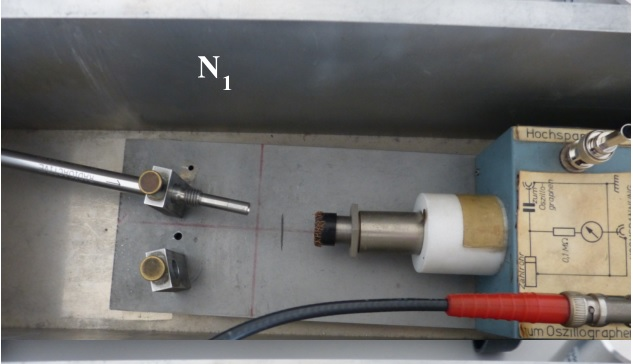
\includegraphics[height=2.5cm]{content/data/N1.jpg}
        \caption{$N_1$}
        \label{fig:N1}
    \end{subfigure}
    \begin{subfigure}{0.3\textwidth}
        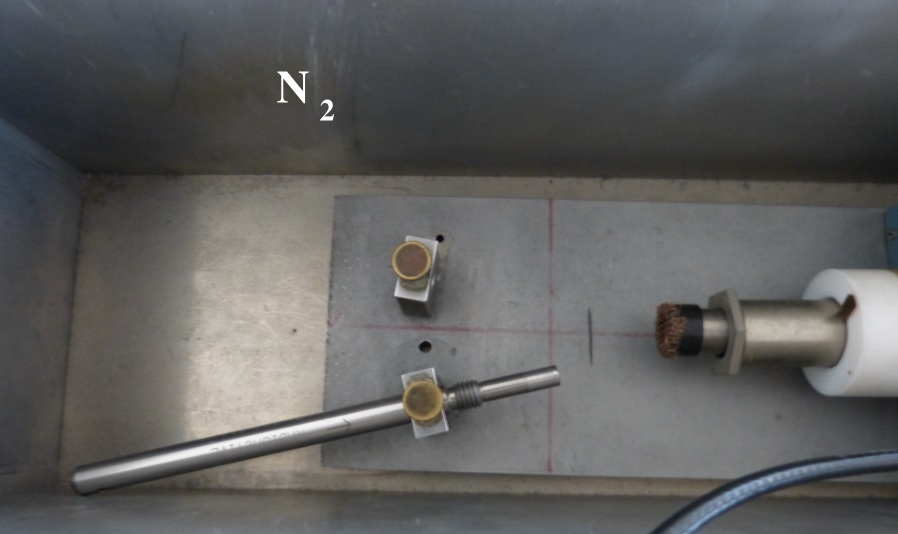
\includegraphics[height=2.5cm]{content/data/N2.jpg}
        \caption{$N_{1+2}$}
        \label{fig:N12}
    \end{subfigure}
    \begin{subfigure}{0.3\textwidth}
        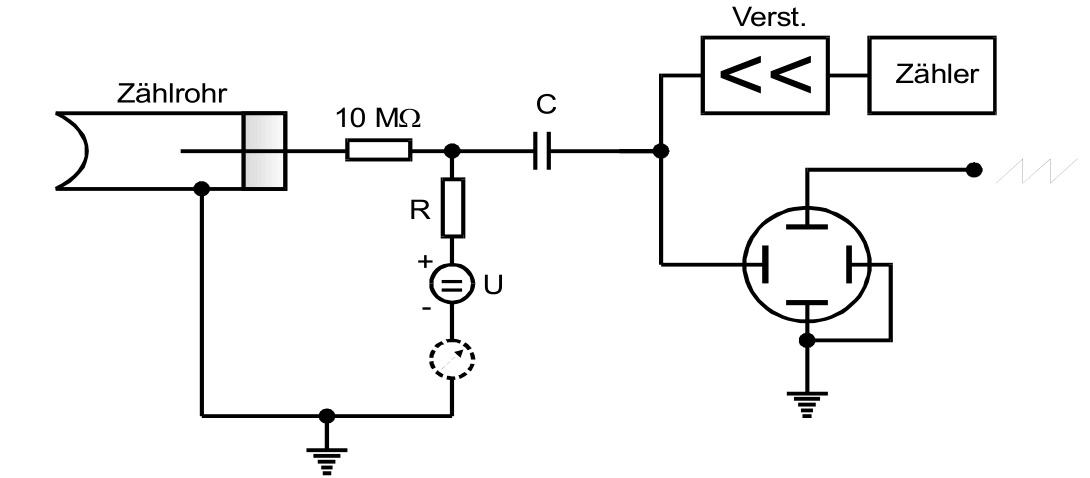
\includegraphics[height=2.5cm]{content/data/aufbau.jpg}
        \caption{$N_2$}
        \label{fig:N2}
    \end{subfigure}
    \caption{Aufbau zur Messung der Totzeit mit der Zwei-Quellen-Methode. \cite[2]{hinweise}}
    \label{fig:zweiquelle}
\end{figure}
Wenn $N_{1+2} < N_1 + N_2$ so hat das Zählrohr eine Totzeit $T$.
Die Totzeit kann nach
\begin{equation}
    T \approx \frac{N_1 + N_2 - N_{1+2}}{2 \cdot N_1 N_2}
    \label{eqn:totzeit}
\end{equation}
angenähert werden.
Die Näherung ist für $T^2 N_i^2 << 1$ mit $i = 1, 2, 1+2$ gültig.